%%%%%%%%%%%%%%%%%%%%%%%%%%%%%%%%%%%%%%%%%%%%%%%%%%%%%%%%%%%%%%%%%%%%%%%%%%%%%%%%
%2345678901234567890123456789012345678901234567890123456789012345678901234567890
%        1         2         3         4         5         6         7         8

%\documentclass[letterpaper, 10 pt, conference]{ieeeconf}  % Comment this line out
                                                          % if you need a4paper
\documentclass[a4paper, 10pt, conference]{ieeeconf}      % Use this line for a4
                                                          % paper

\IEEEoverridecommandlockouts                              % This command is only
                                                          % needed if you want to
                                                          % use the \thanks command
\overrideIEEEmargins
% See the \addtolength command later in the file to balance the column lengths
% on the last page of the document



% The following packages can be found on http:\\www.ctan.org
\usepackage{graphicx} % for pdf, bitmapped graphics files
%\usepackage{epsfig} % for postscript graphics files
%\usepackage{mathptmx} % assumes new font selection scheme installed
%\usepackage{times} % assumes new font selection scheme installed
%\usepackage{amsmath} % assumes amsmath package installed
%\usepackage{amssymb}  % assumes amsmath package installed

%-Para bash and c++
\usepackage{listings}

%-Hrefs
\usepackage{hyperref}

\makeatletter
\def\BState{\State\hskip-\ALG@thistlm}
\makeatother


\title{\LARGE \bf
Practical Tutorial for SDR using GNU Radio
}

%\author{ \parbox{3 in}{\centering Huibert Kwakernaak*
%         \thanks{*Use the $\backslash$thanks command to put information here}\\
%         Faculty of Electrical Engineering, Mathematics and Computer Science\\
%         University of Twente\\
%         7500 AE Enschede, The Netherlands\\
%         {\tt\small h.kwakernaak@autsubmit.com}}
%         \hspace*{ 0.5 in}
%         \parbox{3 in}{ \centering Pradeep Misra**
%         \thanks{**The footnote marks may be inserted manually}\\
%        Department of Electrical Engineering \\
%         Wright State University\\
%         Dayton, OH 45435, USA\\
%         {\tt\small pmisra@cs.wright.edu}}
%}


\author{André Silva$^{1}$
\thanks{*This work was supported by Instituto de Telecomunicações}% <-this % stops a space
\thanks{$^{1}$André Silva is with Faculty of Sciences and Technology,
        University of Coimbra, Portugal}
}

\begin{document}

\maketitle
\thispagestyle{empty}
\pagestyle{empty}


%%%%%%%%%%%%%%%%%%%%%%%%%%%%%%%%%%%%%%%%%%%%%%%%%%%%%%%%%%%%%%%%%%%%%%%%%%%%%%%%
\begin{abstract}

This electronic document is a ÒliveÓ template. The various components of your paper [title, text, heads, etc.] are already defined on the style sheet, as illustrated by the portions given in this document.

\end{abstract}


%%%%%%%%%%%%%%%%%%%%%%%%%%%%%%%%%%%%%%%%%%%%%%%%%%%%%%%%%%%%%%%%%%%%%%%%%%%%%%%%
\section{INTRODUCTION}

SOMETHING

\section{GETTING STARTED}
We need a Linux base for getting started, this installing guide was meant to Ubuntu 18.04 or the Ubuntu 19.04.
\subsection{Installing VOLK}
First of all we will install VOLK (Vector-Optimized Library of Kernels) because we will not use the internal VOLK of GNU Radio but an external one. VOLK it's a free library that contains kernels for mathematical operations, this means that for an operation is created a proto-kernel and added to VOLK for the architecture that we wish, hence faster operations. To install this follow the next commands:

\begin{lstlisting}[language=bash, breaklines]
$git clone https://github.com/gnuradio/volk
$cd volk && mkdir build && cd build
$cmake ../ && make && make test
$sudo make install && sudo ldconfig
\end{lstlisting}

To complete this, we need to create a profile for our architecture, for this go to \verb|/usr/bin/| folder and run \verb|./volk_profile|. Note that the configuration file is written in the next path: \verb|$HOME/.volk/volk_config|.

\subsection{Installing GNU Radio}
Now moving for GNU Radio, the first thing to do is install all the dependencies needed, with the next command:
\begin{lstlisting}[breaklines]
sudo apt install cmake git g++ libboost-all-dev python-dev python-mako python-numpy python-wxgtk3.0 python-sphinx python-cheetah swig libzmq3-dev libfftw3-dev libgsl-dev libcppunit-dev doxygen libcomedi-dev libqt4-opengl-dev python-qt4 libqwt-dev libsdl1.2-dev libusb-1.0-0-dev python-gtk2 python-lxml pkg-config python-sip-dev
\end{lstlisting}

After dependencies installed we will install GNU Radio via git. It is available the Version 3.8 however still has a lot of stability problems and bugs so we keep with the last commit of 3.7 version:
\begin{lstlisting}[language=bash, breaklines]
$git clone https://github.com/gnuradio/gnuradio.git
$cd gnuradio && git checkout maint-3.7
$mkdir build && cd build
$cmake -DENABLE_INTERNAL_VOLK=OFF ../
$make && make test && sudo make install && sudo ldconfig
\end{lstlisting}

You can now use the GNU Radio, to see where was installed where it is a usefull command: "which gnuradio-companion".

\subsection{Installing UHD Driver}
To use the USRP's we need to install the UHD Driver, and for that we install three packages:
\verb|libuhd-dev, libuhd3.14.1| and \verb|uhd-host|.
This packages can be downloaded here:
\url{https://launchpad.net/~ettusresearch/+archive/ubuntu/uhd/+packages}.

Finally to download the image of your USRP just run: 
\verb|./uhd_images_downloader.py| inside the folder \verb|/usr/lib/uhd/utils/|.

If everything works you can run the next command to see the devices connected:
\verb|$uhd_find_devices|, and this one to see information about that devices: \verb|$uhd_usrp_probe"|.


\subsection{Problems and Solutions}
After installing GNU Radio when you open it if shows some warnings about \verb|Camberra| just install it with:.
\begin{lstlisting}[language=bash, breaklines]
$sudo apt install libcanberra-gtk-module libcanberra-gtk3-module
\end{lstlisting}


\section{GUIDED TUTORIAL - MODULATION}

BALBLABLA

\subsection{Modulation - Tutorial\_1.grc}
    In order to transmit data between SDR's it's necessary modulate the signal, so the modulation is the act of varying properties of a waveform, this wave is called carrier and keeps the information transmitted, so the the goal here is pick the data and modulate it so it can be transmitted in single carrier.
    
    First we need to understand the working of some blocks and hence the GNU Radio itself. 
    
    %-----------
    
    We can convert bytes in complex numbers using the "Chunks to Symbols" block, this block has a parameter called "Symbol Table" where we define the mapping between a byte (a chunk, this is our symbol) and a constellation point (point in the constellation to the symbol). But before we need to do two things:
        First we need to unpack the byte, this means split the 8 bits/byte in X significant bits/byte where X is the number of bits necessary to the symbol of the constellation type, this is, if we want modulate in BPSK X is 1, QPSK X is 2, 8PSK X is 4.
        This is possible using the "Repack Bits" block, this block has 3 important parameters, the "Bits per Input Byte" where we define how many bits we pick in an incoming byte, the "Bits per Output Byte" where we define how many significant bits will have the output byte (the remaining bits will be 0's), and finally the parameter "Endianness" to determinate if we want write in MSB or LSB (always read in LSB). 
    
    For example if we input the byte = "01000010":
    
    With 8:2 in MSB we got:"000000\textbf{01}", "000000\textbf{00}", "000000\textbf{00}", "000000\textbf{10}".
    
    With 8:2 in LSB we got:"000000\textbf{10}", "000000\textbf{00}", "000000\textbf{00}", "000000\textbf{01}".
    
    Note that this block leads to an interpolation of "Bits per Output Byte/Bits per Input Byte, in this case 8/2=4, this is, for every 1 bytes outputs 4 bytes". 
        
        Second we need to map the resulting bits in the symbols that we really want, using the "Map" block that basically does: \verb|output[i] = map[input[i]]|.
    
    Lets suppose we want modulate using QPSK: 
        First we create an "Constellation Object" where we insert the mapping of the symbols relative to the constellation points. 
        We need to pick the 8 bits/byte and slicing in 2 significant bits per byte, so we use the "Repack bits" with 8 "Bits per Input Byte" and 2 "Bits per output Byte" with MSB endianness. Currently we have a byte with the first 6 bits with 0's and the next 2 bits with 2 bits of data, however it's not our symbol yet).
        Then we map this significant 2 bits into the symbol we want taking into account that we will map this symbols in constellation points next (using the "Constellation object" block). In this case the 2 significant bits coincide with the symbol, but it depends of what you want to do.
        Resulting in mapping into the constellation points in the \ref{fig:mapping_qpsk}
        \begin{figure}
            \centering
            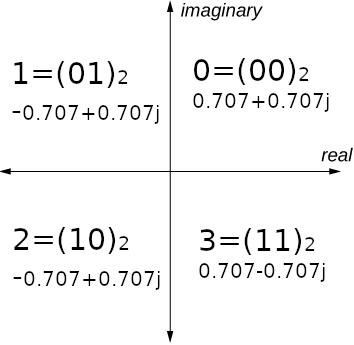
\includegraphics[width=0.75\linewidth]{mapping_qpsk.jpg}
            \caption{QPSK: Mapping Symbols to Constellation Points}
            \label{fig:mapping_qpsk}
        \end{figure}
        
        The last block is "Throttle", to understand this block we need understand how GR works. When we do data streaming, we are implicitly using a buffers to hold the data between blocks, this buffers are in finite size, so before the block do anything, it checks the amount of available space in input and output buffers, if there is none available space in that buffers the block don't do anything. This is called "Back-pressure" because we pressure back the data that is incoming, slowing things down. This is how GR controls the data flow, giving data to the block when it's necessary and holding it when block is busy working. We have source/sink blocks that produces/consumes data at a given fixed sample rate like Audio and USRP blocks, these blocks are called "clock" blocks, so typically a FG has only one source or one sink block, and not both because that leads to an problem called as "2 clock problem" where there is 2 blocks with different sample rates leading a asynchronous clock sources causing "underruns"/"overflows" depending on the production/consumption rates are differentiating. As our FG doesn't has any of this "clock" blocks then we need to add the "Throttle" block to act as a clock, without it the FG will run as fast as the CPU can process resulting in non-responsive program and other problems. This means that while we are in simulating mode we need this block to control the flow however when we start using the "USRP" blocks we can take out this block.
        
        To finalize the TX side we send the data to an virtual sink, that redirects the data to the virtual source with the same id, the only purpose of this block it's make the FG more clear, elegant and readable.
        
        Now we move to the RX part of the FG where we use the "Constellation Decoder" to invert what we have done, this is, map the complex points to symbols (using the parameters of the "he "Constellation Object" block), and then we use "Map" block again to map symbols into bits of real data. And then pick the 2 significant bits and pack in a byte exactly the inverse as before.
        
        
\subsection{Modulation - Tutorial\_2.grc}
    What we have done is not enough because in real world we cant use all the bandwidth, so we need no narrow it, however if the channels are too narrow the symbols will be too wide and the tail of the last symbol will interfere with the present one inducing ISI (Inter-Symbol Interference). A pulse shaping filter we can use to work around is the RRC (Root Raised Cosine) filter because it's a feasible solution and it's implemented in GR.      
    
    %--------RRC filter
   If we don't put a shaping filter on the signal, the waves will have a lot of energy in adjacent channels. This filter uses taps to apply against our signal shaping it. This taps are calculated based in how many number of filters we want and how many samples we want per symbol. Theoretically has an infinite number of taps hence we can infinite attenuate the stop band, so really we can define the limit according with processing power we have. Remember that we have added ISI here that we will have to treat in RX side, as we will see.
   

    %Roll off
    
    Another thing to keep in mind is the roll-off factor, this is the measure of the excess bandwidth of the filter (bandwidth that is occupied beyond Nyquist bandwidth). This parameter is basically the inclination of the wave when rising and falling, when we set more roll-off, let's say 1, then will be easier for the receiver to decode however we will narrow less the bandwidth and that is not our objective, on the other hand, smaller roll-off will result in narrower bandwidth, however the inclination increases so attenuation in stop band is reduced.
    I provide an FG that made called "roll\_off.grc" inside of "extra" folder where you can analyse the plot of 5 different roll-off factors. In this tutorial we will use the 0.22 value to this parameter.
    %-filter delay.
    %--Decreasing the number of samples (filter delay) reduces the stop band attenuation.
    
    %---SPS
    Another thing included in modulation is the interpolation, so basically we can set a number of SPS (samples per symbol) that we want however, logically, more samples per symbol leads to less probability of errors hence inducting more overhead to our transmission. What this does is construct new points in the wave between the existing ones thus when we will reconstruct the signal we will be a lot more precise. To find this parameter we have 2 criteria:  First leaving this values small as possible taking into account that is mandatory to be 2 or higher. Second we can use this value to help us match the desired bit rate taking into account the sample rate of the hardware we are using, (currently none but we will use USRP's). We will use 4 for this parameter.
    
    %--------RX SIDE - chega??
    Note that at this point we have ISI in our signal, so first I have to get rid of this by using another RRC filter. When we combine 2 RRC filter together we get a RRC filter with Nyquist filter form. Knowing this property we can use another RRC filter resulting in a raised cosine pulse shaped filter with less ISI. If you observe the constellation plot "RX Treated Constellation" there is a little noisy as a result of the ISI after the 32 filters however much less noisy than "RX Constellation". 
    %--SPS 4-1
    
    Now that we have applied a RRC filter to our RX signal, in the same way that we have re-sampling by 4 we need to decimate to converting 4 samples per symbol into only 1 sample per symbol.

\subsection{Modulation - Tutorial\_3.grc}
    Now we are ready no get closer to reality, for that let's implement a "Channel Model" block where simulates different properties of a channel that we will need to take care:
    
\begin{itemize}
\item Noise - We can add Additive White Gaussian Noise (AWGN) in parameter "Noise Voltage" where we set a level as a voltage;
\item Frequency Offset - The "Frequency\_offset" parameter where 0 is no offset and 0.25 would be a digital modem (1/4 of the symbol rate);
\item Timing Offset - The "Epsilon" parameter allows emulating different sample clocks between the transmitter e the receiver and 1.0 is no offset added.
\item Multipath - We can emulate multipath delay by adding taps of a FIR (Finite Impulse Response) filter in the "Taps" parameter.
\end{itemize}
    
    
    The FG we have is already taken care of noise and timing offset using the "Polyphase Clock Sync" block. If you play with the tweaks "Time Offset" and "Noise Amp" you can see in the plot of "Rx Treated constellation" a nice and clear constellation, however if you tweak the "Freq Offset" you can see that the constellation become a circle, that's because we are not treating that, it will be what we will do next tutorial.
    
\subsection{Modulation - Tutorial\_4.grc}
    %O que é multipath - tratar MULTIPATH
    Multipath is having different paths to our receptor like when we are using wireless the signal  reflects on objects of the environment, for example walls, and go to receptor a little after the direct path, so the receptor receives the same signal various times with timing differences. 
    I added some taps to simulate a multipath property, if you disable "Costas Loop" and the "CMA Equalizer" and set "Output SPS" to 1 in the "Polyphase Clock Sync" block you can see the effect of these taps because the constellation points are no longer clean and really converged: Fig: \ref{fig:multipath_effect}

    \begin{figure}
        \centering
        \includegraphics[width=\linewidth]{multipath_effect.png}
        \caption{Effects Multipath on Constellation Plot}
        \label{fig:multipath_effect}
    \end{figure}
    
    This, obviously affects our transmission so to take out this problem we will need an equalizer, called "CMA equalizer". Here we define the number of taps where more taps means better final results however more overhead to the algorithm thus we want keep this number small but enough for correcting our channel (based on educated guess, I set 15 because works with other implementations and is enough for now). The "Gain" I set 0.01 and the "Samples per Symbol" of the input signal is set to "2", hence, the "Output SPS" of "Polyphase Clock Sync" block is also set to "2". If you take a look now for the constellation plot you will see a constellation a lot more converged and clean: Fig: \ref{fig:multipath_corrected}

    \begin{figure}
        \centering
        \includegraphics[width=\linewidth]{multipath_corrected.png}
        \caption{Multipath corrected on Constellation Plot}
        \label{fig:multipath_corrected}
    \end{figure}
    
    %TRATAR Frequency offset - COSTAS LOOP -------__MELHORAR??????????
    Note that the constellation is rotating a little, the "CMA Equalizer" all it cares about is converging in a unit circle without any knowledge of the constellation, so when it locks, locks in a given phase, thus we need to take care of the phase offset. Besides that, if you tweak the "Freq Offset" you will see an circle instead a constellation, that is why we need to take care of the last property mentioned before: "Frequency offset".
    We can track the offset of both of this things using an second order loop, however this type of recover is "fine frequency correction" this means that we need to be close of the ideal frequency or our constellation won't converge and will keep spinning. 
    We have to set the "Loop bandwidth" and the "Order" parameters, the first one is relative to the second order loop (I will use 6.28/200.0), the second is about the order of the constellation type (2 to BPSK, 4 to QPSK and 8 to 8PSK, thus 4 for our example). Now you can enable this block you will note that the constellation is no more rotating and if you tweak the Frequency Offset note that it's not getting a circle anymore, instead that, the constellation keeps without rotation, clear and converged.  

\subsection{Modulation - Tutorial\_5.grc}
    If you take a closer look we have an problem writing the file, sometimes writes something and another times doesn't. That's because we might have an ambiguity of 90 degrees in our constellation. The solution for this is: Instead transmitting constellation itself, we will transmit the difference between symbols of the constellation, and then mapping the transmitted symbols into our bits of data. Basically the differential encoding depends not only of the transmitted symbol but also the previous one, removing ambiguity of 90 degrees. If it's the case of BPSK we would have 180 degrees of ambiguity, if it's 8PSK it would be 45 degrees of ambiguity.
    In our FG we can resolve by adding an "Differential Encoder" Block right after "Map" block resulting in first mapping the bits of data in symbols, and then convert these symbols in differential symbols dependent of the last one, and finally convert to constellation symbols. 
    In RX is just do the inverse thing, right after we have the transmitted symbols we use "Differential Decoder" to get the real symbols and then map to the bits of data.
    
    
\subsection{Packet communications - Tutorial\_6.grc}
    %---Header e CAC
    Now we have successfully modulated and transmitted our signal without ambiguity, but if you take a look in the output file, it will only be junk. This is happening because it's not writing the bits in the supposed byte. Explaining better, if I send the byte "01010101" and for some motive receives 4 bits in 0's and then the right byte, this results in "0000\textbf{0101}" and "\textbf{0101}XXXX", then all the bits forward are not aligned. This is the problem that is happening here because the "Polyphase Clock Sync" block needs some time to adapt and in this time losses some bits, so we need a manner to always receive the bytes aligned. The solution for this is packetize our data and send the packet, consequently, we will lose all that packet but we will always get our bits aligned.
    
    %CAC
    The first thing we need to know is how the "Correlate Access Code - Tag Stream" block works. It expect unpacked data, this means that the input only has 1 significant bit per byte. Then exams the input finding an sequence called "Access Code" of 64 bits taking into account that can be X bits different where X is the "Threshold" parameter. After find this sequence the next 16 bits is the length of the payload (that will be outputted) repeated twice (32 bits in total). Resulting in a header with 64 bits of access code, 16 bits of payload length and another 16 bits of payload length, being that the length of the payload is in bytes. Now that we have the composition of the header of the packet we need to create it.
    
    %Inicio
    Assuming that we want transmit packets with 112 bytes of payload size, hence 896 bits, then we need to create the header with that information. 
    %-Create header
    To create the header we will use the "Vector Source" block with the "Repeat" parameter set to "Yes", and the vector will be 64 bits of the access code (I will use the default that can be accessed here "digital.packet\_utils.default\_access\_code"), followed by "00000000 01110000" = 112 and then "00000000 01110000" = 112. With header ready we need to split the input in 1 bit/byte using "Repack Bits" block mentioned before, then concatenate the 96 bits of the header with 896 bits of the payload using "Stream Mux" block, and finally repack again to 2 bits/byte resulting in the packet ready to modulate and transmit. Of course that this can be optimized by instead repacking into 1 bits, uses directly 2 bits and creating the header with that in mind, but I am splitting in 1 bit because we will use FEC (Forward Error Correction) encoding ahead.
    
    %RX
    At the RX side we just need to repack to the 2 bits/byte into 1 bit/byte to use the "Correlate Access Code - Tag Stream" block and extract the payload of the packet and finally repack to 8 bits/byte. Now if you take a look at the output file you see that the bits are aligned correctly in the byte needed.
    
\subsection{Out-Of-Tree Modules - Tutorial\_7.grc}
    We are getting the bits aligned, but we lose the first packet so we can solve this by transmitting an vector of bits right before we transmit our real data. There is just a big problem: the GR doesn't has that implemented but has a thing called OOT (Out-Of-Tree Modules) where allow us extend GR with our own functions and blocks created in python or in C++. Now I will teach how to create a block in GR: The first thing is going to an folder where you want keep the OOT blocks and run the following commands: 

\begin{lstlisting}[language=bash, breaklines]
$gr_modtool newmod insert_vec_cpp
$cd gr-insert_vec_cpp
$gr_modtool add new_vec
\end{lstlisting}

    Now we need to chose the type of block we want to write, where:
    \begin{itemize}
        \item Source - With this blocks you can produce output items.
        \item Sink - With this blocks you can consume input items.
        \item General -This block is a general version, where you can define the rate of consumption/production. 
        \item Interpolator/Decimator - Use this type when you want a fixed multiple rate of consumption/production.
        \item Hier - This is called "Hierarchical blocks" where you can aggregate multiple existing blocks in one block. You can also do this in a graphical way on GR by setting the parameter "Generate Options" as a "Hier Block" located in Options of the FG.
        \item No Block - You can also create FG without any graphical blocks, only code.
    \end{itemize}
    
    For our purpose I selected \verb|general|, and then we need to select the language (it can be in Python or C++), I have selected \verb|cpp| as the language, then you need to input the arguments that your block will take, as I want only an vector of bytes I put \verb|const std::vector<unsigned char> &vec|, and  finally you select if you want QA (Quality Assurance) code, this is a template where you can do unit testing on your code (I selected no).
    
    Here it's created 3 important things:
\begin{verbatim}
File 'lib/new_vec_impl.h'
File 'lib/new_vec_impl.cc'
File 'grc/insert_vec_cpp_new_vec.xml'
\end{verbatim}

    The first one is the header file of our source code file witch is the second file and where we will write our code. The last one is an XML file where we link our code to the GR.
    
    %---CODE
    Let's carefully analyse the source file:
\begin{lstlisting}[language=c++, breaklines]
gr::io_signature::make(<+MIN_IN+>, <+MAX_IN+>, sizeof(<+ITYPE+>)),
gr::io_signature::make(<+MIN_OUT+>, <+MAX_OUT+>, sizeof(<+OTYPE+>)))
\end{lstlisting}

    The GR adds \verb|<+| and \verb|+>| in places that you need to replace for values that you need. In the first line is where you select how many input connections you need, namely the minimum number, the maximum number, and the size of the type of data that will be on that connections. In our case we want to get in only one connection (so min=1 and max=1) and treat like a byte, this means that we need to set an \verb|unsigned char|.
    The second line is where you select how many output connections you need, namely the minimum number, the maximum number, and the size of the type of data that will be in each connection, so it's exactly the same as before.
    
    Besides that we will need to use our vector in another function (general\_work), an flag to know if all the vector was sent and finally an index to track how many bits of the vector we already sent.
    Resulting in changes in file source and header file, in file source just add this:
\begin{lstlisting}[language=c++, breaklines]   
gr::io_signature::make(1, 1, sizeof(unsigned char)),
gr::io_signature::make(1, 1, sizeof(unsigned char))),
d_data(vec),
flag(0),
track_oo(0)
\end{lstlisting}  

    In header file declare the variables:
\begin{lstlisting}[language=c++, breaklines] 
    std::vector<unsigned char> d_data;
    int flag;
    int track_oo;
\end{lstlisting} 
    And make getters and setters:
    
 \begin{lstlisting}[language=c++, breaklines]   
void set_data(const std::vector<unsigned char> &vec){
    d_data=vec;}
int get_flag(){
    return flag;}
void set_flag(){
    flag=1;}
void set_track(int a){
    track_oo=a;}
int get_track(){
    return track_oo;}
\end{lstlisting}    

    The next function to treat in file source is this one:
\begin{lstlisting}[language=c++, breaklines]   
teste_impl::forecast (int noutput_items, gr_vector_int &ninput_items_required){}
\end{lstlisting}
    
    Here is where you define the production/consumption rate you want. We will want 1:1 so you need to add this in that function:
    
\begin{lstlisting}[language=c++, breaklines]    
unsigned ninputs = ninput_items_required.size();
for(unsigned i = 0; i < ninputs; i++)
    ninput_items_required[i] = noutput_items;
\end{lstlisting}
    
    Moving on for the core work \verb|general_work()| that will be performed by the block, the template show us this:

\begin{lstlisting}[language=c++, breaklines]    
    const <+ITYPE+> *in = (const <+ITYPE+> *) input_items[0];
    <+OTYPE+> *out = (<+OTYPE+> *) output_items[0];
    consume_each (noutput_items);
    return noutput_items;

\end{lstlisting}

    Again we need to replace content of the \verb|<+| \verb|+>| for our type of data: \verb|unsigned char|. The consume\_each() function is where we set the number of items that we will consumed and at front of the return is the number of items that we produced.
    
    Going for the code itself:
    If all the vector was already inserted, then we just pass through the items doing nothing to them, using the \verb|memcpy()|.
    If there is the first time or vector to send then we need to send it, taking into account that we can only send the maximum size available on the output buffer. In case there is not enough space we sent what we can and update the variable to keep track of the last byte sent and next time we know where we will start sending the vector. Here we don't consume anything, we are just producing items. In case there is enough space then we sent the rest of the vector and set the flag to know that we already sent all the vector and starts passing directly the next items.
    So in \verb|general_work()| we will add this:

\begin{lstlisting}[language=c++, breaklines]
int ii=0;
int oo=0;
if(get_flag()==1){ //Vector already inserted
    ii=noutput_items;
    oo=noutput_items;
    memcpy(&out[0], &in[0], sizeof(unsigned char)*noutput_items);
}
else{ //First time or vector not fully sent, so I need to insert the vector
    int max_copy = std::min (noutput_items, (((int) d_data.size()) - get_track()) ); //Check for space in buffers to use the remaining vector (len(vec) - used)
    oo=max_copy; //That's what I will output (produce, it can be all vector or all buffer)
    ii=0; //I don't want consume anything
    memcpy(&out[0],&d_data[get_track()],sizeof(unsigned char)*max_copy); //Output starting from where I stopped the last time (Starting with 0)
    if(max_copy == (((int) d_data.size()) - get_track()) ){ //If I will use last piece of the vector (len(vec)-used) then I can set the flag to get out. (Start passing directly)
        set_flag();
    }
    set_track(get_track()+oo); //Increment the track to know where to start copying the vector the next time (Where I was plus what I will produce now) 
    }
consume_each (ii);
return oo;
\end{lstlisting}

%-XML
    In remaining file we have a XML where we need to set some things so we can link our written code to GR. The first tricky thing is remove the \verb|\&| on the parameter in \verb|<make>| tag. 
    In \verb|<param>| is where we define the parameter that will be parsed in our GR, so we will replace this piece of the template for this:
\begin{lstlisting}[language=xml, breaklines]
<param>
    <name>Vector</name>
    <key>vec</key>
    <type>int_vector</type>
</param>
\end{lstlisting}
    Then in \verb|<sink>| and in \verb|<souce>| has a parameter called \verb|<type>| where we set what type of data will be inputted and outputted, in this case will be \verb|byte|.

    Now that we have all code written we need compile it and link to our GRC with these commands:
    
\begin{lstlisting}[language=bash, breaklines]
$wget mkdir build && cd build
$cmake ../ && make
$sudo make install
$sudo ldconfig
\end{lstlisting}
    
    Finally we just need to click in "Reload Block" in the toolbar in GR and use the block like any other.
    
\subsection{Forward Error Correction - LDPC - Tutorial\_10_1.grc}
as


\subsection{Forward Error Correction - CC - Tutorial\_10_2.grc}
as

\subsection{Equations}
\subsection{Some Common Mistakes}
\section{USING THE TEMPLATE}

\subsection{Headings, etc}


\subsection{Figures and Tables}

\begin{table}[h]
\caption{An Example of a Table}
\label{table_example}
\begin{center}
\begin{tabular}{|c||c|}
\hline
One & Two\\
\hline
Three & Four\\
\hline
\end{tabular}
\end{center}
\end{table}




\section{CONCLUSIONS}

A conclusion section is not required. Although a conclusion may review the main points of the paper, do not replicate the abstract as the conclusion. A conclusion might elaborate on the importance of the work or suggest applications and extensions. 

\addtolength{\textheight}{-12cm}   % This command serves to balance the column lengths
                                  % on the last page of the document manually. It shortens
                                  % the textheight of the last page by a suitable amount.
                                  % This command does not take effect until the next page
                                  % so it should come on the page before the last. Make
                                  % sure that you do not shorten the textheight too much.

%%%%%%%%%%%%%%%%%%%%%%%%%%%%%%%%%%%%%%%%%%%%%%%%%%%%%%%%%%%%%%%%%%%%%%%%%%%%%%%%



%%%%%%%%%%%%%%%%%%%%%%%%%%%%%%%%%%%%%%%%%%%%%%%%%%%%%%%%%%%%%%%%%%%%%%%%%%%%%%%%



%%%%%%%%%%%%%%%%%%%%%%%%%%%%%%%%%%%%%%%%%%%%%%%%%%%%%%%%%%%%%%%%%%%%%%%%%%%%%%%%
\section*{APPENDIX}

Appendixes should appear before the acknowledgment.

\section*{ACKNOWLEDGMENT}

The preferred spelling of the word ÒacknowledgmentÓ in America is without an ÒeÓ after the ÒgÓ. Avoid the stilted expression, ÒOne of us (R. B. G.) thanks . . .Ó  Instead, try ÒR. B. G. thanksÓ. Put sponsor acknowledgments in the unnumbered footnote on the first page.



%%%%%%%%%%%%%%%%%%%%%%%%%%%%%%%%%%%%%%%%%%%%%%%%%%%%%%%%%%%%%%%%%%%%%%%%%%%%%%%%

References are important to the reader; therefore, each citation must be complete and correct. If at all possible, references should be commonly available publications.



\begin{thebibliography}{99}

\bibitem{c1} G. O. Young, ÒSynthetic structure of industrial plastics (Book style with paper title and editor),Ó    in Plastics, 2nd ed. vol. 3, J. Peters, Ed.  New York: McGraw-Hill, 1964, pp. 15Ð64.
\bibitem{c2} W.-K. Chen, Linear Networks and Systems (Book style).  Belmont, CA: Wadsworth, 1993, pp. 123Ð135.
\bibitem{c3} H. Poor, An Introduction to Signal Detection and Estimation.   New York: Springer-Verlag, 1985, ch. 4.
\bibitem{c4} B. Smith, ÒAn approach to graphs of linear forms (Unpublished work style),Ó unpublished.
\bibitem{c5} E. H. Miller, ÒA note on reflector arrays (Periodical styleÑAccepted for publication),Ó IEEE Trans. Antennas Propagat., to be publised.
\bibitem{c6} J. Wang, ÒFundamentals of erbium-doped fiber amplifiers arrays (Periodical styleÑSubmitted for publication),Ó IEEE J. Quantum Electron., submitted for publication.
\bibitem{c7} C. J. Kaufman, Rocky Mountain Research Lab., Boulder, CO, private communication, May 1995.
\bibitem{c8} Y. Yorozu, M. Hirano, K. Oka, and Y. Tagawa, ÒElectron spectroscopy studies on magneto-optical media and plastic substrate interfaces(Translation Journals style),Ó IEEE Transl. J. Magn.Jpn., vol. 2, Aug. 1987, pp. 740Ð741 [Dig. 9th Annu. Conf. Magnetics Japan, 1982, p. 301].
\bibitem{c9} M. Young, The Techincal Writers Handbook.  Mill Valley, CA: University Science, 1989.
\bibitem{c10} J. U. Duncombe, ÒInfrared navigationÑPart I: An assessment of feasibility (Periodical style),Ó IEEE Trans. Electron Devices, vol. ED-11, pp. 34Ð39, Jan. 1959.
\bibitem{c11} S. Chen, B. Mulgrew, and P. M. Grant, ÒA clustering technique for digital communications channel equalization using radial basis function networks,Ó IEEE Trans. Neural Networks, vol. 4, pp. 570Ð578, July 1993.
\bibitem{c12} R. W. Lucky, ÒAutomatic equalization for digital communication,Ó Bell Syst. Tech. J., vol. 44, no. 4, pp. 547Ð588, Apr. 1965.
\bibitem{c13} S. P. Bingulac, ÒOn the compatibility of adaptive controllers (Published Conference Proceedings style),Ó in Proc. 4th Annu. Allerton Conf. Circuits and Systems Theory, New York, 1994, pp. 8Ð16.
\bibitem{c14} G. R. Faulhaber, ÒDesign of service systems with priority reservation,Ó in Conf. Rec. 1995 IEEE Int. Conf. Communications, pp. 3Ð8.
\bibitem{c15} W. D. Doyle, ÒMagnetization reversal in films with biaxial anisotropy,Ó in 1987 Proc. INTERMAG Conf., pp. 2.2-1Ð2.2-6.
\bibitem{c16} G. W. Juette and L. E. Zeffanella, ÒRadio noise currents n short sections on bundle conductors (Presented Conference Paper style),Ó presented at the IEEE Summer power Meeting, Dallas, TX, June 22Ð27, 1990, Paper 90 SM 690-0 PWRS.
\bibitem{c17} J. G. Kreifeldt, ÒAn analysis of surface-detected EMG as an amplitude-modulated noise,Ó presented at the 1989 Int. Conf. Medicine and Biological Engineering, Chicago, IL.
\bibitem{c18} J. Williams, ÒNarrow-band analyzer (Thesis or Dissertation style),Ó Ph.D. dissertation, Dept. Elect. Eng., Harvard Univ., Cambridge, MA, 1993. 
\bibitem{c19} N. Kawasaki, ÒParametric study of thermal and chemical nonequilibrium nozzle flow,Ó M.S. thesis, Dept. Electron. Eng., Osaka Univ., Osaka, Japan, 1993.
\bibitem{c20} J. P. Wilkinson, ÒNonlinear resonant circuit devices (Patent style),Ó U.S. Patent 3 624 12, July 16, 1990. 






\end{thebibliography}




\end{document}
